\documentclass[twoside, a4paper, 11pt]{article}
\usepackage[utf8x]{inputenc}
\usepackage[T1]{fontenc}
\usepackage{times}
\usepackage{anysize}
\usepackage{fancyhdr}
\usepackage{pdfpages}
\usepackage{tabularx}

\marginsize{3cm}{2cm}{2cm}{2cm}

% Indicador completo en lugar de página
\fancyfoot[C]{{\ttfamily RTF CU:2.0 \quad \thepage}}
\renewcommand*{\headrulewidth}{0pt}
\pagestyle{fancy}

% Comando para indicar los problemas
\newcommand{\problema}[2]{\begin{description} \item[Exposición] #1 \item[Resolución] #2 \end{description}}

\begin{document}
	% Título
	\begin{center}
		\scshape \large Acta de la Revisión Técnica Formal \textit{Casos de uso} - Grupo Diedral \vspace{.5cm}
	\end{center}

	Reunidos Cristina Alonso Fernández, Juan Andrés Claramunt Pérez y Rubén Rafael Rubio Cuéllar como representantes de la parte revisada, el Grupo Diedral; y Aitor Alonso Lorenzo %, Asier Cardoso Sánchez
y David Roldán Santos por la parte revisora, el equipo Nameless; en el laboratorio 10 de la Facultad de Informática de la Universidad Complutense de Madrid a viernes 8 de marzo de 2013 a las 14:00, se procede a la Revisión Técnica Formal del documento ``Casos de uso'' con número de registro CU:2.0 perteneciente al Grupo Diedral.\\

	El equipo revisor presenta un documento, anexo a al presente, con sus conclusiones previas. Se tratan los siguientes temas por orden de aparición:

	\begin{enumerate}
		\renewcommand*{\theenumi}{P\arabic{enumi}}
		
		\item \problema{Los tiempos verbales en los enunciados de los casos de uso carecen de coherencia. Ciertos casos han sido expresamente reseñados.}{El Grupo Diedral reconoce el error y se compromete a su corrección.}
		\item \problema{El equipo revisor sugiere indicación explícita en caso de que alguno de los campos de las tablas de descripción de casos de uso quedase vacío.}{No se llega a ninguna conclusión al considerarse el asunto de escasa relevancia.}
		\item \problema{Se sugiere poner como precondición una conexión estable a la base de datos para así ahorrar numerosas secuencias alternativas.}{Se toma la sugerencia en consideración, si bien no se admite en principio puesto que la existencia de una conexión estable con la base de datos durante todo el desarrollo del caso de uso puede ser una exigencia irrealizable, y en todo caso inverificable a priori.}
		\item \problema{Ciertos diagramas contienen nombres de casos de uso que no se corresponden exactamente con el nombre dado en la descripción. Es más, algunos casos de uso descritos no aparecen en el diagrama.}{El equipo de desarrollo admite que los diagramas están desactualizados y se compromete a su reparación.}
		\item \problema{El equipo revisor afirma que tanto \textit{Registrar Empleado} como \textit{Dar de baja empleado}, que en el diagrama extienden al caso \textit{Acceder}, no tienen ninguna relación con el caso \textit{Acceder} y por tanto debería eliminarse la relación del diagrama.}{No se llegó a acuerdo en este asunto.}
		\item \problema{La parte revisora sugiere la eliminación o fusión del caso \textit{Verificar registro de empleado} con el caso de uso \textit{Registrar empleado}.}{Se rechaza esa sugerencia porque la política de privilegios de usuario y supervisión escogida para el proyecto demanda su existencia, pero se considera explicar de forma más clara en el documento dicha circunstancia, que por otro lado está desarrollada en otros \mbox{documentos} del proyecto.}
		\item \problema{El caso \textit{Configurar sistema general} no especifica los parámetros configurables.}{Se admite el error y se acuerda su corrección.}
		\item \problema{El equipo revisor afirma que en el c.u. \textit{Establecer organización laboral} no se llega nunca a la secuencia alternativa S-1. Algo semejante ocurre en el caso \textit{Acceder horarios} y \textit{Consultar plan de vuelo}.}{La parte revisada admite que no se ha hecho mención explícita a la correspondiente secuencia alternativa en la secuencia normal, si bien la propia secuencia alternativa indica explícitamente bajo que circunstancias acontece. Los errores serán corregidos.}
		\item \problema{Se sugiere incluir el caso \textit{Acceder horarios} en ver \textit{Consultar ficha empleado} o fusionarlos.}{Se explica que el caso \textit{Consultar ficha empleado} es una caso que corresponde en principio al personal de Recursos Humanos de la compañía aérea, mientras que el caso \textit{Acceder horarios} tiene como principal objetivo permitir la consulta por parte de cada empleado de su horario personal, por lo que la sugerencia no tiene mucho sentido. Se considera mejorar la claridad de la exposición.}
		\item \problema{En el caso \textit{Introducir plan de vuelo} la secuencia S-1 adolece de sentido.}{Se admite el error y queda pendiente de corregir.}
		\item \problema{Se hace constar que en ciertos casos de uso aparece en lugar del texto correspondiente el término `\textit{postexito}'.}{Se trata de un error sintáctico del sistema tipográfico, anteriormente corregido en la versión entregada al profesor en formato electrónico.}
		\item \problema{En la secuencia alternativa S-1 de \textit{Modificar inventario} se tacha de incorrecta la redacción.}{Se reredactará el texto señalado.}
		\item \problema{En \textit{Modificar inventario} no se indica a qué parte de la secuencia normal lleva el reintento de la secuencia alternativa S-3.}{Se considera reescribir el citado punto, si bien el punto de retorno parecería ser el punto que conduce a la secuencia alternativa.}
		\item \problema{Se sugiere contar con una cola de acciones pendientes para intentos fallidos de comunicación.}{Se desestima por los conflictos que podría acarrear y su inconveniencia para la integridad de la información manipulada, dado que no se asegura la vuelta al funcionamiento del equipo local donde se almacene dicha cola.}
		\item \problema{Diferentes casos de despistes en la redacción que aparecen reseñados en el documento adjunto como faltas de ortografía.}{Se corregirán.}
		\item \problema{En \textit{Registrar entrada de material} el equipo revisor admite que no se entiende bien, hasta el punto de afirmar que pudiera ser redundante con el caso \textit{Modificar inventario}. También se dice que la ``impresión del adhesivo'' es un problema del \textit{hardware} que no debería aparecer en ese documento.}{El equipo revisado se compromete a estudiar cómo mejorar la redacción de ese apar\-tado y explica su significado para justificar su valor como caso de uso. La impresión de un \mbox{`adhesivo'} (tal vez no específicamente un adhesivo) es relevante pues impone un requisito de manejo de periféricos de impresión al \textit{software}.}
		\item \problema{\textit{Programar oferta} es totalmente ambiguo.}{Se admite y se compromete su arreglo.}
		\item \problema{\textit{Ver incidencias del sistema} no indica las secuencias alternativas, hipotecándolas a las propias del método de acceso al servidor.}{El caso \textit{Ver incidencias del sistema} no indica más que la posibilidad de ver los \mbox{registros} que han sido generados por el software como archivos de texto plano en el sistema de archivos del servidor donde opera. Las secuencias alternativas son exclusivamente consecuencia del método de acceso a los archivos en dicho servidor, en ese caso, los \mbox{desarrolladores}, con la venia del cliente, se reservan el derecho a no especificarlos explícitamente.}
		\item \problema{Problemas de nombres y relaciones en los diagramas de gestión externa.}{No se llegó a acuerdo con las relaciones. Los conflictos de nombres serán resueltos.}
		\item \problema{Problemas con la impresión de la tarjeta de embarque entre los casos relacionados con la adquisición de billetes.}{Se estudiará y acometerá el correcto acople de los antedichos casos.}
	\end{enumerate}

	\vspace*{1cm}

	Quedan de acuerdo sobre la fidelidad de estos puntos a los hechos acaecidos en la fecha y lugar anteriormente reseñados, el Grupo Diedral y Nameless, por vía de sus representantes.\\

	% Espacio para las firmas
	\begin{tabularx}{.9\linewidth}{X  >{\raggedleft}X}
		El Grupo Diedral & Nameless
	\end{tabularx}

	% Indica que viene el anexo
	\vfill{}
	{\itshape A continuación se incluye el anexo elaborado por el equipo revisor:}

	% Incluye el anexo del otro grupo
	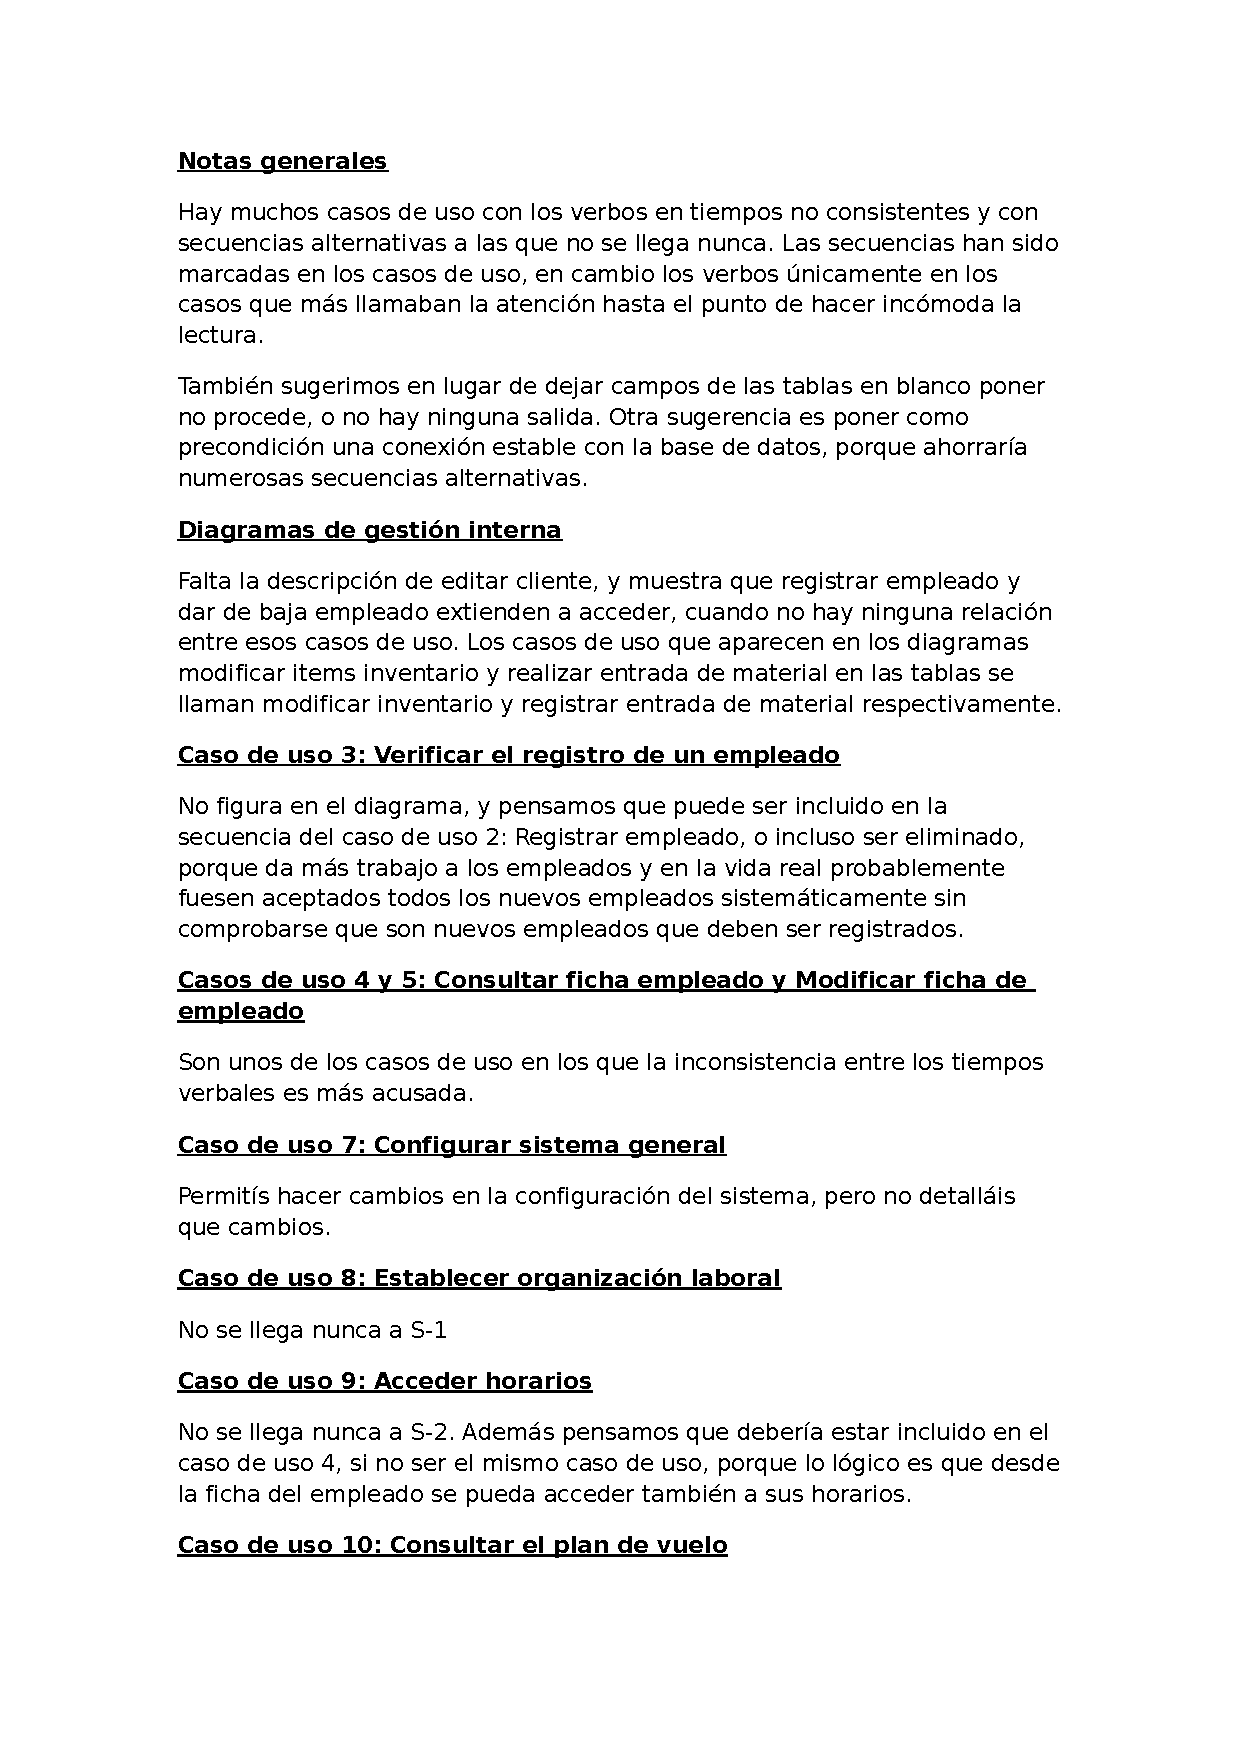
\includepdf[pages=1-3, pagecommand={}]{RevisionDiedral.pdf}
\end{document}
